% questions.tex —— 1977 年·贵州卷 · 题目内容片段（无答案）
% 由 tools/generate_projects.py 依来源总账自 1977/1977_数学真题_贵州_试题.md 生成，勿手改（改源 MD 后重跑）


\gkpart{贵州1977年高考数学试题解}

\begin{gktip}
\textbf{来源说明}：本题面依据固定源 PDF《贵州1977年高考数学试题解》第 1—6 页（书籍页码 135—140）逐题转录。固定源是题面与解答连续出现的扫描材料，而不是无答案试卷；配套答案与解析对照源解答独立复算，非官方标准答案。卷首注明「文科考生只作前 5 题，理科考生 8 题全作」，故科类栏记为文理合卷。正式题为第一大题至第八大题，其中第一、二两大题各含 2 个小题，源卷小题印作「1．、2．」，本库按小问规范重排为（1）（2）；末尾「参考题」2 道由考生选作（25 岁以上的考生必作），不计入题量。源卷排印用字「园」（圆）、「叙列」（数列）照录。
\end{gktip}

\par\medskip

\begin{question}
\gkti{1}将下列各式化成最简形式：

（1） $\sqrt[4]{a^{-2}b^{3}}\cdot\sqrt[3]{a^{4}b^{-2}}\div\sqrt[6]{a^{5}\cdot b^{-2}}$

（2） $\operatorname{Log}_2\cos\dfrac{\pi}{4}-\operatorname{Log}_2\sin\dfrac{\pi}{6}$

\end{question}
\begin{question}
\gkti{2}计算下列各题：

（1） 已知 $\operatorname{tg}\alpha=\dfrac{2ab}{a^{2}-b^{2}}$，求 $\sin\alpha$。

（2） 已知：$m+\dfrac{1}{m}=2$，求 $m^{2}+\dfrac{1}{m^{2}}=?\qquad m^{3}+\dfrac{1}{m^{3}}=?$

\Needspace{0.4\textheight}
\end{question}
\begin{question}
\gkti{3}以直角三角形 $ABC$ 的一直角边 $AB$ 为直径作园，此园与斜边 $AC$ 交于 $D$，过 $D$ 引园的切线交 $BC$ 于 $E$。试证：$EB=CE$。

\begin{gktip}
原源 PDF 第 3 页附有直角三角形、以直角边为直径的园与过 $D$ 的切线示意图（含 $\angle1$—$\angle4$ 标注与虚线 $BD$）；LaTeX 版按源图重绘。
\end{gktip}
\nopagebreak[4]
\begin{center}% 1977 年贵州卷第三题：直角三角形 ABC（∠ABC=90°），以直角边 AB 为直径作园，
% 园与斜边 AC 交于 D，过 D 的切线交 BC 于 E（切线向 D 上方延长），
% 虚线为辅助线 BD；角标注 ∠1（CDE）、∠2（DCE）、∠3（EDB）、∠4（DBE），
% B 处另画直角记号（按源卷第 3 页布局，几何关系自洽：ED=EB=3）
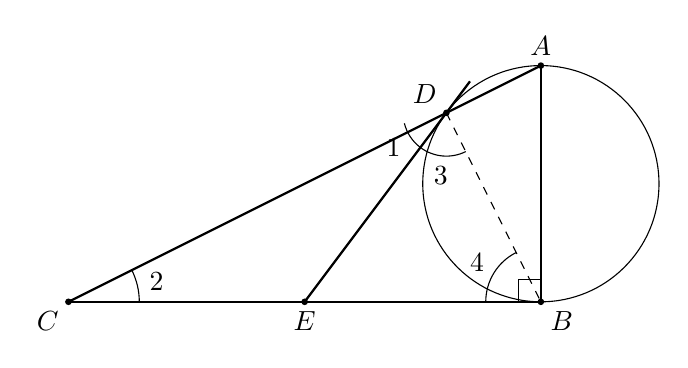
\begin{tikzpicture}[scale=1.0]
  \coordinate (B) at (0,0);
  \coordinate (A) at (0,3);
  \coordinate (C) at (-6,0);
  \coordinate (O) at (0,1.5);
  \coordinate (D) at (-1.2,2.4);
  \coordinate (E) at (-3,0);
  \coordinate (T) at (-0.9,2.8);
  \draw (O) circle (1.5);
  \draw[thick] (C)--(A);
  \draw[thick] (A)--(B);
  \draw[thick] (C)--(B);
  \draw[thick] (E)--(T);
  \draw[dashed] (D)--(B);
  \fill (A) circle (1.2pt) node[above] {$A$};
  \fill (B) circle (1.2pt) node[below right] {$B$};
  \fill (C) circle (1.2pt) node[below left] {$C$};
  \fill (D) circle (1.2pt) node[above left] {$D$};
  \fill (E) circle (1.2pt) node[below] {$E$};
  % ∠2（C 处，CB 与 CA 之间）
  \draw ([shift={(0:0.9)}]C) arc (0:26.57:0.9);
  \node at (-4.88,0.26) {$2$};
  % ∠1（D 处，DC 与 DE 之间）
  \draw ([shift={(194.04:0.55)}]D) arc (194.04:233.13:0.55);
  \node at (-1.87,1.96) {$1$};
  % ∠3（D 处，DE 与 DB 之间）
  \draw ([shift={(233.13:0.55)}]D) arc (233.13:296.57:0.55);
  \node at (-1.27,1.60) {$3$};
  % ∠4（B 处，BD 与 BC 之间）
  \draw ([shift={(116.57:0.7)}]B) arc (116.57:180:0.7);
  \node at (-0.81,0.50) {$4$};
  % B 处直角记号（∠ABC=90°）
  \draw (0,0.28)--(-0.28,0.28)--(-0.28,0);
\end{tikzpicture}
\end{center}
\nopagebreak[4]
\end{question}
\begin{question}
\gkti{4}求到点 $A(1,2)$ 和点 $B(4,1)$ 等距离的点的轨迹的方程。

\end{question}
\begin{question}
\gkti{5}用长 $8$ 米的木料，做一矩形的窗框，问长和宽如何选择，才能使窗子透过的光线最多？

\end{question}
\begin{question}
\gkti{6}求 $\operatorname{Lim}_{n\to\infty}a\sin\alpha\left(1+\cos\alpha+\cos^{2}\alpha+\cdots+\cos^{n}\alpha\right)=?$（其中 $a$ 为任意实常数，$0<\alpha<\dfrac{\pi}{2}$）

\end{question}
\begin{question}
\gkti{7}已知方程 $x^{2}+px+q=0$ 的两个根为 $\operatorname{tg}\alpha$ 与 $\operatorname{tg}\beta$，求

\nopagebreak[4]
\[
\sin^{2}(\alpha+\beta)+p\sin(\alpha+\beta)\cos(\alpha+\beta)+q\cos^{2}(\alpha+\beta)
\]

的值，（其中 P、q 为任意实常数）。

\begin{gktip}
\textbf{源注}：括注中的大写「P」系源卷排印（题中系数实为 $p$），照录。
\end{gktip}

\Needspace{0.4\textheight}
\end{question}
\begin{question}
\gkti{8}设有直线（L）与曲线（c）：直线（L）：$y=ax-1$；曲线（c）：$r\sin\theta=\sin2\theta$。问（L）与（c）在什么条件下相交、相切、不相交。

\textbf{参考题 1．} 设某平板上任意一点的电势，在 $\rho\geqslant1$ 时，由 $E=\operatorname{Ln}\rho$ 给出，这里 $\rho$ 是以原点为起点的矢径。试求在点 $\rho=5$，$C-\arcsin 0.8$ 处，沿此点至 $\rho=10$，$\theta=\dfrac{\pi}{2}$ 的方向 $E$ 的变化率。

\begin{gktip}
\textbf{源注}：源卷题面印作「C—arcsin0.8」；同页解答及答句均作「$\theta=\arcsin 0.8$」（对应直角坐标点 $(3,4)$），「C—」系「$\theta=$」的排印误植，题面照录原样并在此说明。
原源 PDF 第 5 页附有直角坐标系、点 $(3,4)$、$(0,10)$ 与方向向量 $\vec{l}$ 的示意图；LaTeX 版按源图重绘。
\end{gktip}
\nopagebreak[4]
\begin{center}% 1977 年贵州卷参考题一：直角坐标系、刻度、单位向量 i 与 j、
% 点 (3,4) 与 (0,10)、虚线向两轴投影、方向向量 l 从 (3,4) 指向 (0,10)
% （按源卷第 5 页布局）
\begin{tikzpicture}[>=stealth,scale=0.85]
  \draw[->] (-0.7,0)--(7,0) node[below] {$x$};
  \draw[->] (0,-0.7)--(0,11) node[left] {$y$};
  \foreach \t in {2,4,6} \draw (\t,0.12)--(\t,-0.12) node[below] {$\t$};
  \foreach \t in {2,4,6,8,10} \draw (0.12,\t)--(-0.12,\t) node[left] {$\t$};
  % 单位向量
  \draw[->,thick] (0,0)--(0.9,0);
  \node at (0.5,-0.55) {$\vec{i}$};
  \draw[->,thick] (0,0)--(0,0.9);
  \node at (-0.55,0.5) {$\vec{j}$};
  % 虚线投影
  \draw[dashed] (3,0)--(3,4)--(0,4);
  % 方向向量
  \draw[->,very thick] (3,4)--(0,10);
  \node at (1.95,6.9) {$\vec{l}$};
  \fill (3,4) circle (2pt) node[right] {$(3,4)$};
  \fill (0,10) circle (2pt) node[above right] {$(0,10)$};
  \node at (0,0) [below left] {$0$};
\end{tikzpicture}
\end{center}
\nopagebreak[4]
\Needspace{5\baselineskip}
\textbf{参考题 2．} 证明

\nopagebreak[4]
\[
S_{1}=1,\quad S_{2}=1+\frac{1}{2^{2}},\quad S_{3}=1+\frac{1}{2^{2}}+\frac{1}{3^{2}},\ \cdots,\quad S_{n}=1+\frac{1}{2^{2}}+\frac{1}{3^{2}}+\cdots+\frac{1}{n^{2}},\ \cdots
\]

是收敛叙列。

\begin{gktip}
\textbf{源注}：源卷首项印作「S,=1」，系下标 1 误印为逗号，本文按 $S_{1}=1$ 转录；「叙列」为源卷排印用字，照录。
\end{gktip}

\end{question}